\section{Protein polymer synthesis---Titin I27}
\label{sec:polymer-synthesis}

Early experiments in force spectroscopy involved
DNA\citep{bustamante94,florin95}, but before long they were also
investigating proteins.  Native titin was one of the first proteins
studied with force spectroscopy\index{titin}\citep{rief97a}.  Titin is
a muscle protein involved in passive elasticity
(\cref{fig:skeletal-muscle}), so it is an ideal subject when examining
the effect of mechanical force\citep{labeit95}.  Titin is also
interesting because, while it is one of the largest known proteins, it
is composed of a series of globular domains.  When \citet{rief97a}
carried out their seminal unfolding experiment, they observed a very
characteristic sawtooth as the domains unfolded (see
\cref{sec:procedure} for a discussion of these sawteeth).

\begin{figure}
  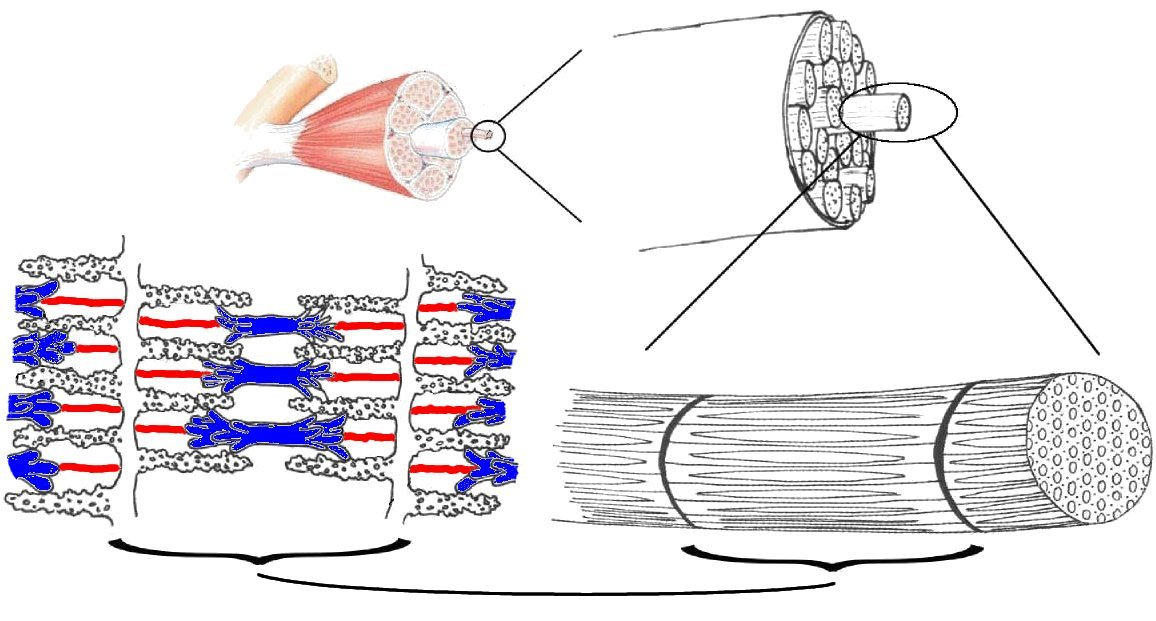
\includegraphics[width=0.7\textwidth]{figures/binary/skeletal_muscle}%
  \caption{Biological role of titin\index{titin}.  Moving clockwise
    from the upper left you can see a bone/muscle group, a muscle
    fiber, a myofibril, and a sarcomere.  In the sarcomere, the white,
    knobbly filaments are actin.  The myosin bundles are blue, and the
    titin linkers are red.  When the muscle contracts, the myosin
    heads walk up the actin filiaments, shortening the sarcomere.
    When the muscle relaxes, the myosin heads release the actin
    filimants and slide back, lengthening the sarcomere.  Titin
    functions as an entropic spring that keeps the myosin from falling
    out of place during the passive, relaxed stage.  This figure is
    adapted from \citet{skeletal_muscle}.\label{fig:skeletal-muscle}}
\end{figure}

Unfortunately, it is difficult to analyze the unfolding of native
titin, because the heterogenous globular domains make it hard to
attribute a particular subdomain to a partuclar unfolding event.
Unfolding a single domain is not feasable because the large radius of
curvature of an AFM tip ($\sim20\U{nm}$\citep{olympus-tr400psa})
dwarfs the radius of a globular domain
($\sim2\U{nm}$\citep{improta96}).  When such a large tip is so close
to the substrate, van der Waals forces and non-specific binding with
the surface dominate the tip-surface interaction.  In order to
increase the tip-surface distance while preserving single molecule
analysis, \citet{carrion-vazquez99b} synthesized a protein composed of
eight repeats of immunoglobulin-like domain 27 (I27\index{I27}), one
of the globular domains from native titin (\cref{fig:I27}).  Octameric
I27 produced using their procedure is now available
commercially\citep{athenaes-i27o}.
%
\nomenclature[text ]{I27}{Immunoglobulin-like domain 27 from human
  titin.}

\begin{figure}
  \includegraphics[width=2in]{figures/i27/1TIT}
  \caption{I27, the immunoglobulin-like domain 27 from human titin
    (\href{http://dx.doi.org/10.2210/pdb1tit/pdb}{PDB ID: 1TIT})%
    \citep{improta96}.  The entire domain is $4.7\U{nm}$ from end to
    end.  Figure generated with \citetalias{pymol}.
    \label{fig:I27}\index{I27}}
\end{figure}

Synthetic proteins are generally produced by creating a plasmid coding
for the target protein, inserting the plasmid in a bacteria, waiting
while the bacteria produce your protein, and then purifying your
proteins from the resulting culture.  In this case,
\citet{carrion-vazquez99b} extracted messenger RNA coding for titin
from human cardiac tissue\citep{rief97a}, and used reverse
transcriptase to generate a complementary DNA (cDNA) library from
human cardiac muscle messenger RNA.  This cDNA is then amplified using
the polymerase chain reaction (PCR), with special primers that allow
you to splice the resulting cDNA into a plasmid (which ends up with
one I27).  Then they ran another PCR on the plasmid, linearized the
plasmid with two restriction enzymes, and grafted two I27-containing
sections together to form a new plasmid (now with two I27s,
\cref{fig:plasmid}).  Another PCR-split-join cycle produced a plasmid
with four I27s, and a final cycle produced a plasmid with eight.  The
eventual plasmid vector has the eight I27s and a host-specific
promoter that causes the bacteria to produce large quantities of I27.
The exact structure of the generated octamer
is\citep{carrion-vazquez99b}
\nomenclature[text ]{cDNA}{Complementary DNA.}
\nomenclature[text ]{PCR}{Polymerase chain reaction.}

\begin{center}
  Met-Arg-Gly-Ser-(His)$_6$-Gly-Ser-(I27-Arg-Ser)$_7$-I27-\ldots-Cys-Cys
  \label{eq:I27}
\end{center}

\begin{figure}
  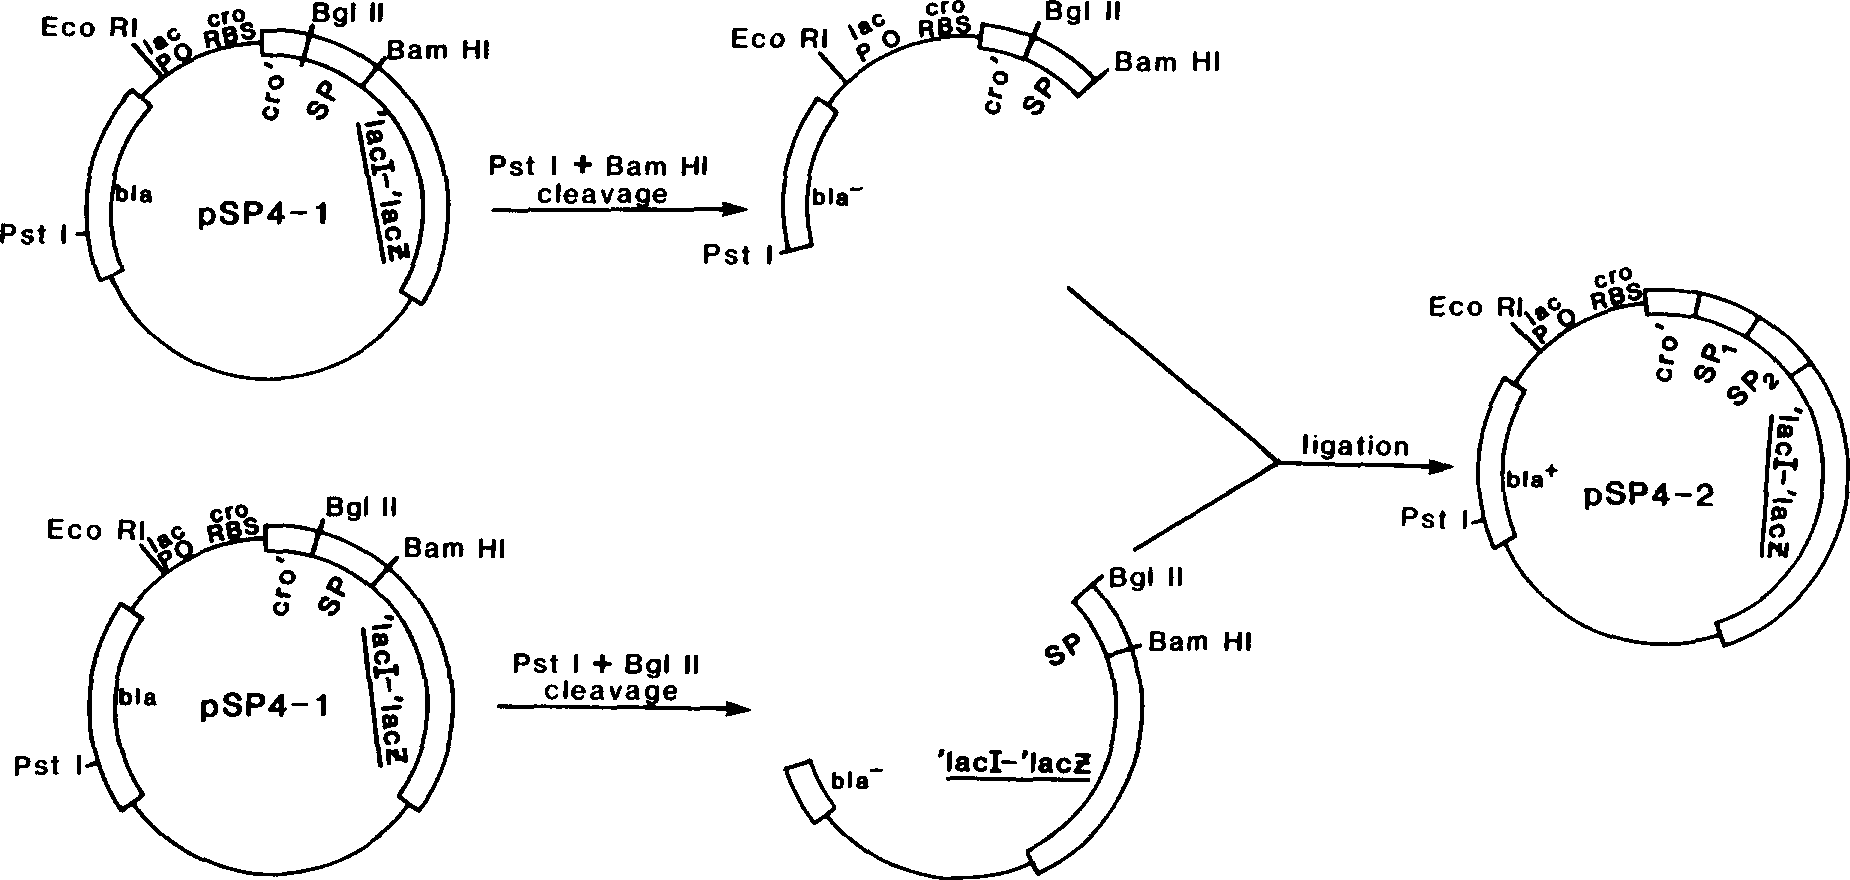
\includegraphics[width=0.9\textwidth]{figures/binary/kempe85-fig2}%
  \caption{Example of gene duplication via plasmid splicing
    (\xref{kempe85}{figure}{2}).  \citet{kempe85} use a different
    gene, but some of the restriction enzymes are shared with
    \citet{carrion-vazquez99b}.  The overall approach is
    identical.\label{fig:plasmid}}
\end{figure}

\index{\species{Escherichia coli}}
The plasmid is then transformed into the host, usually
\species{Escherichia coli}\citep{carrion-vazquez99b,bartels03,ma10} or
a proprietary equivalent such as Agilent's SURE 2 Supercompetent
Cells\citep{agilent-sure2,carrion-vazquez00}.  The infected cells are
cultured to express the protein.
%
\nomenclature[text ]{Bacterial transformation}{The process by which
  bacterial cells take up exogenous DNA molecules.}
\nomenclature[text ]{Exogenous DNA}{DNA that is outside of a cell.}

The octamer is then purified from the culture using immobilized metal
ion affinity chromatography (IMAC), where the His-tagged end of the
octamer covalently bonds to a metal ion that is bound to the column
media (e.g. Ni-NTA\index{Ni-NTA} coated
beads)\citep{carrion-vazquez00,bartels03,ma10}.  Once the rest of the
broth has been washed out of the chromatography column, the octamer is
eluted via either another molecule which competes for the metal
ions\citep{ma10} or by changing the pH so the octamer is less
attracted to the metal ion.
%
\nomenclature[text ]{IMAC}{Immobilized metal ion affinity
  chromatography.}
\nomenclature[text ]{Ni-NTA}{Nickle nitrilotriacetic acid.}

\nomenclature[text ]{Ala}{Alanine, an amino acid.}
\nomenclature[text ]{Arg}{Arginine, an amino acid.}
\nomenclature[text ]{Asn}{Asparagine, an amino acid.}
\nomenclature[text ]{Asp}{Aspartic acid, an amino acid.}
\nomenclature[text ]{Cys}{Cystine, an amino acid.}
\nomenclature[text ]{Glu}{Glutamic acid, an amino acid.}
\nomenclature[text ]{Gln}{Glutamine, an amino acid.}
\nomenclature[text ]{Gly}{Glycine, an amino acid.}
\nomenclature[text ]{His}{Histidine, an amino acid.}
\nomenclature[text ]{Ile}{Isoleucine, an amino acid.}
\nomenclature[text ]{Leu}{Leucine, an amino acid.}
\nomenclature[text ]{Lys}{Lysine, an amino acid.}
\nomenclature[text ]{Met}{Methionine, an amino acid.}
\nomenclature[text ]{Phe}{Phenylalanine, an amino acid.}
\nomenclature[text ]{Pro}{Proline, an amino acid.}
\nomenclature[text ]{Ser}{Serine, an amino acid.}
\nomenclature[text ]{Thr}{Threonine, an amino acid.}
\nomenclature[text ]{Trp}{Tryptophan, an amino acid.}
\nomenclature[text ]{Tyr}{Tyrosine, an amino acid.}
\nomenclature[text ]{Val}{Valine, an amino acid.}
